% disc.tex

\chapter{Discrétisation}

\section{Notations}

\subsection{Cadre en dimension 1}
\label{sec:notation_1D}

On considère $\Omega = [a,b]$, $a<b$, un intervalle de $\mathbb{R}$ de longueur $L=b-a$. Dans la suite, nous utilisons les lettres latines pour noter les fonctions continues : $f(x)$, $u(x)$, ... $x \in \Omega$. Si $u$ et $v$ sont des fonctions définies sur $\Omega$, leur produit scalaire dans $L^2 ( \Omega )$ est donné par :
\begin{equation}
(u,v) = \gint_{\Omega} u(x) \bar{v}(x) dx = \gint_{a}^b u(x) \bar{v}(x) dx.
\end{equation}
Nous travaillerons, sauf mention contraire, avec des fonctions à valeurs dans $\mathbb{R}$. Dans ce cadre, le produit scalaire devient :
\begin{equation}
(u,v) = \gint_{a}^b u(x) v(x) dx.
\end{equation}
La norme sur $L^2(\Omega)$ est donnée par :
\begin{equation}
\| u \|_{L^2(\Omega)} = \sqrt{(u,u)} = \left( \gint_{a}^b u(x) u(x) dx \right)^{1/2}.
\end{equation}
La norme infinie sur $L^{\infty}(\Omega)$ est donnée par :
\begin{equation}
\| u \|_{\infty} = \sup_{x\in\Omega} |u(x)|.
\end{equation}
On dit qu'une fonction $u : x \in \Omega \mapsto u(x) \in \mathbb{R}$ est \textit{périodique} sur $\Omega$ de période $L$ si pour tout $x \in \Omega$, on a 
\begin{equation}
u(x+L) = u(x).
\end{equation}
En particulier, on a $u(a)=u(b)$. Dans le contexte périodique, on considère que $x_0 = x_N$.

On considère une grille régulière sur $\Omega$ constituée de $N \in \mathbb{N}^{\star}$ points :
\begin{equation}
a=x_0 < x_1 < \ldots < x_{N-1} < x_N = b,
\end{equation}
où les valeurs de $(x_i)_{0\leq i \leq N}$ sont données par :
\begin{equation}
x_i = a + ih\text{, } i = 0,1, \ldots,N \text{ et } h = \dfrac{b-a}{N}. 
\end{equation}

\begin{figure}[htbp]
\begin{center}
\begin{tikzpicture}[scale=1.8]
	\draw [>=stealth, <->] (-2,0.2) -- (-1,.2) ;
	\draw (-1.5,.3) node[above] {$h$} ;
	\draw (-3,0) -- (3,0) ;
	\draw (-3,0) node {$\times$} ;
	\draw (-3,-.2) node[below] {$x_0=a$} ;
	\draw (-2,0) node {$\bullet$} ;
	\draw (-2,-.2) node[below] {$x_1$} ;
	\draw (-1,0) node {$\bullet$} ;
	\draw (-1,-.2) node[below] {$x_2$} ;
	\draw (0,-.2) node[below] {$\ldots$} ;
	\draw (1,0) node {$\bullet$} ;
	\draw (1,-.2) node[below] {$x_{N-2}$} ;
	\draw (2,0) node {$\bullet$} ;
	\draw (2,-.2) node[below] {$x_{N-1}$} ;
	\draw (3,0) node {$\times$} ;
	\draw (3,-.2) node[below] {$x_N =b$} ;
\end{tikzpicture}
\end{center}
\caption{Grille en dimension 1. Les symboles $\times$ désignent les points de bords, les symboles $\bullet$ désignent les points intérieurs de la grille.}
\label{fig:maillage1D}
\end{figure}

Les points $x_0=a$ et $x_N = a + L = b$ désignent les points de bords du domaines alors que les points $(x_i)_{1 \leq i \leq N-1}$ désignent les points intérieurs. Une fonction $x \in \Omega \mapsto u(x)$ est discrétisée par la donnée de ses valeurs en chaque points de grille.
Nous distinguons trois niveaux de représentation des fonctions aux points de grille.
\begin{itemize}
\item On note $\mathfrak{u}$ la \textit{fonction de grille} définie sur la grille discrète $(x_i)_{0 \leq i \leq}$. Les fonctions de grilles seront notées avec cette typographie : $\mathfrak{u}$, $\mathfrak{v}$, ... 
On a alors :
\begin{equation}
\mathfrak{u} = (\mathfrak{u}(x_0), \mathfrak{u}(x_1), \mathfrak{u}(x_2), ... , \mathfrak{u}(x_N)).
\end{equation}
On note $l^2_h$ l'espace des fonctions de grille, $h>0$ fixé.
On munit cet espace d'un produit scalaire et de la norme associée :
\begin{equation}
(\mathfrak{u},\mathfrak{v})_h = h \gsum_{i=0}^N \mathfrak{u}(x_i) \mathfrak{v}(x_i) \text{,  } |\mathfrak{u}|_h^2 = h \gsum_{i=0}^N \mathfrak{u}(x_i)^2.
\end{equation}
On définit aussi la norme infinie pour les fonctions de grille :
\begin{equation}
\| \mathfrak{u} \|_{\infty} = \max_{0\leq i \leq N} |\mathfrak{u}(x_i)|.
\end{equation}

\item Les lettres latines capitales permettent de noter les vecteurs de $\mathbb{R}^{N+1}$ et matrices de $\mathcal{M}_{N+1}(\mathbb{R})$. Par exemple, soit le vecteur $U \in \mathbb{R}^{N+1}$ des composantes de $\mathfrak{u} \in l^2_h$, alors :
\begin{equation}
U = \begin{bmatrix}
\mathfrak{u}_0 \\ \mathfrak{u}_1 \\ \vdots \\ \mathfrak{u}_N
\end{bmatrix} =
\begin{bmatrix}
\mathfrak{u}(x_0) \\ \mathfrak{u}(x_1) \\ \vdots \\ \mathfrak{u}(x_N)
\end{bmatrix}
\end{equation}
La norme Euclidienne sur $\mathbb{R}^{N+1}$ est notée $|U|$. Elle induit une norme pour les matrices $A \in \mathcal{M}_{N+1}(\mathbb{R})$ de taille $(N+1) \times (N+1)$ :
\begin{equation}
|A|_2 = \sup_{U \neq 0} \dfrac{|AU|}{|U|}
\end{equation}
On remarque que si $A$ est symétrique alors :
\begin{equation}
|A|_2 = \rho(A) := \max \left\lbrace |\lambda| \ \lambda \in Sp(A) \right\rbrace.
\end{equation}
$\rho(A)$ est nommé \textit{rayon spectrale} de $A$.
La norme infinie de $U$ est donnée par :
\begin{equation}
|U|_{\infty} = \max_{1 \leq i \leq N+1} |U_i|.
\end{equation}
La norme de $A$ subordonnée à la norme vectorielle infinie est :
\begin{equation}
|A|_{\infty} = \sup_{U \neq 0} \dfrac{|AU|_{\infty}}{|U|_{\infty}} = \max_{1 \leq i \leq N+1} \gsum_{j=1}^{N+1} |A_{i,j}|.
\end{equation}

\item Soit $u: x \in \Omega \mapsto u(x)$, on définit la fonction de grille associée $u^*$ par :
\begin{equation}
u^*_i = u^*(x_i) \text{ pour } 0 \leq i \leq N.
\end{equation}
$u^*$ est la restriction de $u$ aux points de la grille.
\end{itemize}

Dans un contexte périodique, on considère que $x_0 = x_N$.
Nous distinguons $l^2_h$, l'espace des fonctions de grilles, de $\mathbb{R}^{N+1}$ même si ces deux espaces sont isomorphes. Cette distinction permet de faire une claire différences entre :
\begin{itemize}
\item les opérateurs aux différences finies, qui agissent sur les fonctions de grilles,
\item les matrices, qui agissent sur les vecteurs.
\end{itemize}
Les fonctions de grilles contiennent toutes les échelles nécessaires dans le contexte physique alors que les vecteurs sont sans dimension. De plus, le raisonnement au niveau discret est plus naturel avec les fonctions de grilles. Il s'effectue d'une façon abstraite à l'aide d'opérateurs aux différences. En revanche, le codage est effectuée dans le cadre de l'algèbre linéaire.












\subsection{Cadre en dimension 2}
\label{sec:notation_2D}

En dimension 2, les notations sont une extension de celles utilisées en dimension 1. Pour des questions de simplicité, on se limite au cas d'une géométrie carrée. Si $a$ et $b$ sont des réels positifs, nous travaillons dans le carré $\Omega = [a,b]^2$. Chaque côté du carré est de longueur $L=b-a$. 
Soient $u$ et $v$ deux fonctions de $\Omega$ dans $\mathbb{R}$. On définit le produit scalaire usuel dans $L^2 ( \Omega ) $ par :
\begin{equation}
(u,v) = \gint_{\Omega} u(x,y) v(x,y) dx dy.
\end{equation}
La norme associée à ce produit scalaire est :
\begin{equation}
\| u \|_{L^2(\Omega)} = \gint_{\Omega} u(x,y)^2 dx dy. 
\end{equation}
La norme infinie est aussi une norme usuelle sur $L^{\infty}(\Omega)$ :
\begin{equation}
\| u \|_{L^{\infty} ( \Omega )} = \sum_{(x,y) \in \Omega} |u(x,y)|.
\end{equation}
Pour alléger les notations, et lorsque cela ne portera pas à confusions, nous noterons ces deux normes $\| u \|_{L^2}$ et $\| u \|_{L^{\infty}}$.

Dans le domaine $\Omega$, nous construisons une grille constituée des points $(x_i,y_j)_{0 \leq i,j \leq N}$ où $N \in \mathbb{N}^{\star}$ avec $a = x_0 < x_1 < \ldots < x_N = b$ et $a = y_0 < y_1 < \ldots < y_N = b$. Le maillage est régulier donné par $h = \frac{L}{N}$. Les valeurs de $x_i$ et $y_j$ sont données par
\begin{equation}
\left\lbrace\begin{array}{rcl}
x_i & = & a + i h \\
y_j & = & a + j h 
\end{array}\right. \text{ avec } 0 \leq i,j \leq N.
\end{equation}

Les points $(x_i,y_j)_{0 \leq i,j \leq N}$ se divisent en différentes catégories (voir figure \ref{fig:maillage2D}) :
\begin{itemize}
\item Les points de bords lorsque l'on a :
\begin{equation}
i \in \left\lbrace 0 , N \right\rbrace \text{ ou } j \in \left\lbrace 0 , N \right\rbrace,
\end{equation}
\item les points intérieurs lorsque :
\begin{equation}
1 \leq i,j \leq N-1.
\end{equation}
\end{itemize}



\begin{figure}[htbp]
\begin{center}
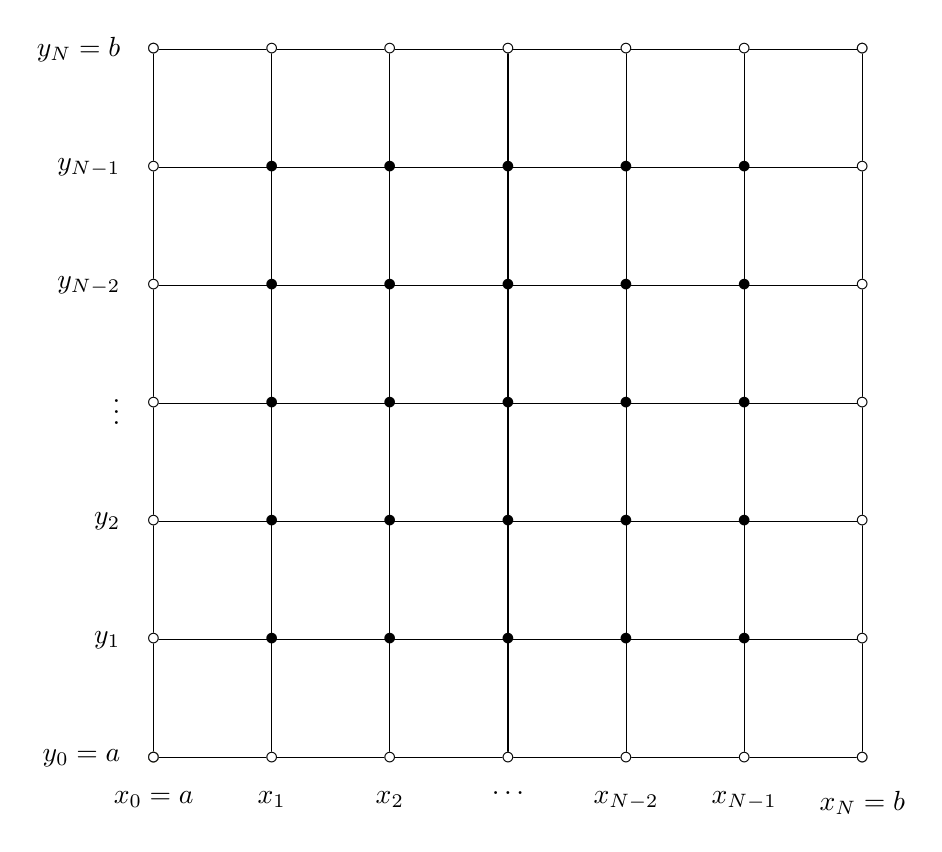
\begin{tikzpicture}[scale=1.5]
	\draw (-3,-3.2) node[below] {$x_0=a$} ;
	\draw (-2,-3.2) node[below] {$x_1$} ;
	\draw (-1,-3.2) node[below] {$x_2$} ;
	\draw (0,-3.2) node[below] {$\ldots$} ;
	\draw (1,-3.2) node[below] {$x_{N-2}$} ;
	\draw (2,-3.2) node[below] {$x_{N-1}$} ;
	\draw (3,-3.2) node[below] {$x_N =b$} ;
	
	\draw (-3.2,-3) node[left] {$y_0=a$} ;
	\draw (-3.2,-2) node[left] {$y_1$} ;
	\draw (-3.2,-1) node[left] {$y_2$} ;
	\draw (-3.2,0) node[left] {$\vdots$} ;
	\draw (-3.2,1) node[left] {$y_{N-2}$} ;
	\draw (-3.2,2) node[left] {$y_{N-1}$} ;
	\draw (-3.2,3) node[left] {$y_N =b$} ;
	
	\draw (-3,-3) grid[step=1] (3,3);

	\draw (-3,-3) node[color=yellow] {$\bullet$} ;
	\draw (-3,-3) node {$\circ$} ;
	
	\foreach \k in {-3,...,3}
		{\draw  (\k,-3) node[color=white] {$\bullet$} ;
	   	\draw (\k,-3) node {$\circ$} ;
	   	\draw  (\k,3) node[color=white] {$\bullet$} ;
	   	\draw (\k,3) node {$\circ$} ;
	   	\draw  (-3,\k) node[color=white] {$\bullet$} ;
	   	\draw (-3,\k) node {$\circ$} ;
	   	\draw  (3,\k) node[color=white] {$\bullet$} ;
	   	\draw (3,\k) node {$\circ$} ;
	   	}
	   	
	\foreach \k in {-2,...,2}
		{\draw  (\k,-2) node {$\bullet$};
		\draw  (\k,-1) node {$\bullet$};
		\draw  (\k,0) node {$\bullet$};
		\draw  (\k,1) node {$\bullet$};
		\draw  (\k,2) node {$\bullet$};
	   	}
\end{tikzpicture}
\end{center}
\caption{Grille en dimension 2. Les symboles $\circ$ désignent les points de bords, les symboles $\bullet$ désignent les points intérieurs de la grille.}
\label{fig:maillage2D}
\end{figure}

On dit qu'une fonction $u : (x,y) \in \Omega \mapsto u(x,y) \in \mathbb{R}$ est \textit{périodique} sur $\Omega$ si 
\begin{equation}
\begin{array}{rcl}
u(x,y+L) & = & u(x,y) \\
u(x+L,y) & = & u(x,y)
\end{array} \text{ pour tous} (x,y) \in \Omega.
\end{equation}

Comme pour le cas en dimension 1, nous définissons différentes notions de fonctions discrètes associées à la grille :
\begin{itemize}
\item Une \textit{fonction de grille} est une fonction définie aux points du maillage $(x_i,y_j)_{0 \leq i,j \leq N}$. Nous notons ces fonctions en gras comme $\mathbf{u}$ ou $\mathbf{v}$. On a :
\begin{equation}
\mathbf{u} = \left( \mathbf{u}(x_i,y_j) \right)_{0 \leq i,j \leq N}.
\end{equation}
$\mathbf{u}$ est périodique si $\mathbf{u}(x_{i},y_0) = \mathbf{u}(x_{i},y_N)$ et $\mathbf{u}(x_{0},y_j) = \mathbf{u}(x_{N},y_j)$ pour tous $0 \leq i,j \leq N$.
On note $L^2_h$ l'espace des fonctions de grilles. Cet espace est équipé d'un produit scalaire et de la norme associée :
\begin{equation}
(\mathbf{u}, \mathbf{v})_h = h^2 \gsum_{i,j=0}^N \mathbf{u}(x_i,y_j) \mathbf{v}(x_i,y_j) \text{ et } |\mathbf{u}|_h = \sqrt{(\mathbf{u},\mathbf{u})_h}.
\end{equation}
La norme infinie de $\mathbf{u}$ est donnée par :
\begin{equation}
| \mathbf{u} |_{\infty} = \max_{0 \leq i,j \leq N} |\mathbf{u}(x_i,y_j)|.
\end{equation}

\item Soit $u : (x,y) \in \Omega \mapsto u(x,y) \in \mathbb{R}$, nous définissons la fonction associée, notée $u^*$ par la restriction de $u$ au maillage :
\begin{equation}
u^*_{i,j} = u(x_i, y_j) \text{ pour tous } 0 \leq i,j \leq N.
\end{equation}

Si $u$ est périodique, on a $u^*_{i,0}=u^*_{i,N}$ et $u^*_{0,j}=u^*_{N,j}$ pour tous $0 \leq i,j \leq N$.
D'une manière générale, dans un contexte périodique, les données sur des bords opposés du carrés coïncident. On considère alors $x_0 = x_N$ et $y_0 = y_N$.
\end{itemize}

\begin{figure}[htbp]
\begin{center}
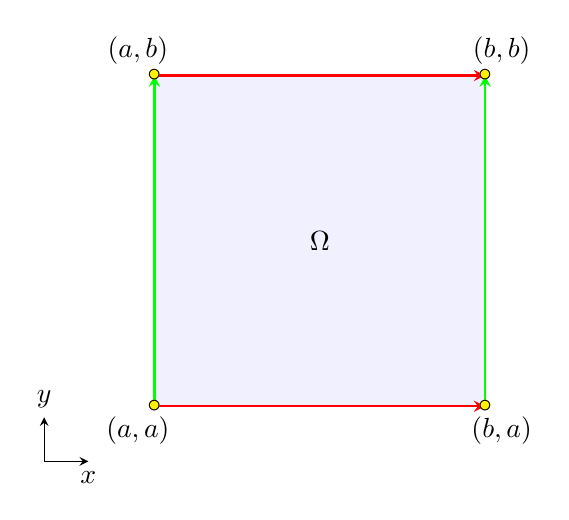
\begin{tikzpicture}[scale=.7]
	\filldraw[draw=black,fill=blue!30!white,opacity=0.20]
	plot (-3,-3) -- (-3,3)
	-- plot (-3,3) -- (3,3)
	-- plot (3,3) -- (3,-3)
	-- plot (3,-3) -- (-3,-3)
	-- cycle;

	\draw [>=stealth, ->,color=green,thick] (-3,-3) -- (-3,3) ;
	\draw [>=stealth, ->,color=green,thick] (3,-3) -- (3,3) ;
	\draw [>=stealth, ->,color=red,thick] (-3,-3) -- (3,-3) ;
	\draw [>=stealth, ->,color=red,thick] (-3,3) -- (3,3) ;
	
	\draw (-3.3,-3.45) node {$(a,a)$} ;
	\draw (3.3,-3.45) node {$(b,a)$} ;
	\draw (-3.3,3.45) node {$(a,b)$} ;
	\draw (3.3,3.45) node {$(b,b)$} ;
	\draw (0,0) node {$\Omega$} ;
	\draw  (-3,-3) node[color=yellow] {$\bullet$} ;
	\draw (-3,-3) node {$\circ$} ;
	\draw  (3,-3) node[color=yellow] {$\bullet$} ;
	\draw (3,-3) node {$\circ$} ;
	\draw  (-3,3) node[color=yellow] {$\bullet$} ;
	\draw (-3,3) node {$\circ$} ;
	\draw  (3,3) node[color=yellow] {$\bullet$} ;
	\draw (3,3) node {$\circ$} ;
	\draw [>=stealth, ->] (-5,-4) -- (-4.2,-4) ;
	\draw (-4.2,-4) node[below] {$x$} ;
	\draw [>=stealth, ->] (-5,-4) -- (-5,-3.2) ;
	\draw (-5,-3.2) node[above] {$y$} ;
\end{tikzpicture}
\end{center}
\caption{Carré périodique. Dans le contexte périodique, les bords de couleurs identiques coïncident. Les quatres coins du carré représentent la même donnée.}
\label{fig:period2D}
\end{figure}









\section{Opérateurs aux différences}

\subsection{Opérateurs classiques périodiques 1D}

On considère $\Omega = [0,L]$. Les notations employées sont celles de la partie \ref{sec:notation_1D} dans le contexte périodique.

\begin{definition}
L'\textit{opérateur de translation} $\tau_p$, $p \in \mathbb{Z}$, est tel que si $\mathfrak{u}$ est une fonction de grille périodique alors pour tout $0 \leq i \leq N$
\begin{equation}
(\tau_p \mathfrak{u})_i = \mathfrak{u}_{i+p}.
\end{equation}
\end{definition}

Cet opérateur permettra de définir les opérateurs aux différences dans la suite. Nous noterons que cet opérateur agit sur les fonctions de grille périodiques $u^*$ par :
\begin{equation}
(\tau_p u^*)_i = u^*_{i+p} = u(x_{i+p}).
\end{equation}
En considérant les propriétés de périodicités si $i+p > N$ ou $i+p<1$.
De la même manière, on définit l'opérateur $\tau$ par 
\begin{equation}
\tau = \tau_{1}
\end{equation}
On note $\tau^p$ où $p$ est un entier naturel 
\begin{equation}
\begin{array}{rcl}
\tau^0 & = & id\\
\tau^p & = & \underbrace{\tau \circ \tau \circ \tau \circ \cdots \circ \tau}_{p \text{ fois.}}
\end{array}
\end{equation}

\begin{proposition}
L'égalité suivante est vérifiée :
\begin{equation}
\tau^p = \tau_p
\end{equation}
\end{proposition}

\begin{proof}
Résultat vrai par récurrence immédiate.
\end{proof}
Il est intéressant de recherches les valeurs propres et les vecteurs propres de $\tau$ de manière à en déduire le spectre des opérateurs qui sont issus de $\tau$.


\begin{proposition}
Les fonctions propres de $\tau$ sont les fonctions de grilles $\mathfrak{u}^k$ vérifiant :
\begin{equation}
\mathfrak{u}_j^k = \exp \left[ i j \dfrac{2 \pi k}{N} \right]
\label{eq:vecteurpropre_tau}
\end{equation}
Chaque vecteur propre est associé à la valeur propre $\lambda^k$ avec 
\begin{equation}
\lambda = \exp \left[ i \dfrac{2 \pi}{N} \right].
\end{equation}
avec $0 \leq k \leq N-1$.
\end{proposition}


\begin{proof}
On calcule $(\tau \mathfrak{u}^k)_j$ :
\begin{equation}
(\tau \mathfrak{u}^k)_j = \exp \left[ i (j+1) \dfrac{2 \pi k}{N} \right] = \exp \left[ i j \dfrac{2 \pi k}{N} \right] \exp \left[ i \dfrac{2 \pi k}{N} \right]  = \mathfrak{u}^k \lambda^k
\end{equation}
De plus, il est facile de voir que $\mathfrak{u}$ vérifie l'hypothèse de périodicité, d'où le résultat.
\end{proof}
Si $P(x)$ est un polynôme en $x$, \textit{i.e.} $P \in \mathbb{R}_{N-1} [x]$ alors les valeurs propres de $P(\tau)$ sont connues :

\begin{proposition}
Les vecteurs propres de $P(\tau)$ sont les fonctions de grilles $\mathfrak{u}^k$ vérifiant :
\begin{equation}
\mathfrak{u}_j^k = \exp \left[ i j \dfrac{2 \pi k}{N} \right]
\end{equation}
Chaque vecteur propre est associé à la valeur propre $P(\lambda^k)$ avec 
\begin{equation}
\lambda = \exp \left[ i \dfrac{2 \pi}{N} \right]
\end{equation}
avec $0 \leq k \leq N-1$.
\label{prop:eigen_tau}
\end{proposition}

\begin{proof}
Soient $(a_i)_{0 \leq i \leq N-1}$ des réels tels que 
\begin{equation}
P(x) = \gsum_{i=0}^{N-1} a_i x^i,
\end{equation}

Calculons $P(\tau) \mathfrak{u}^k$. Soit $j$ un entier compris entre $0$ et $N-1$, 

\begin{equation}
(P(\tau) \mathfrak{u}^k)_j = \left( \gsum_{i=0}^{N-1} a_i \tau_ p \mathfrak{u}^k \right)_j = \gsum_{i=0}^{N-1} a_i (\lambda^k)^p \mathfrak{u}^k_j = P(\lambda^k) \mathfrak{u}^k_j
\end{equation}

d'où le résultat.
\end{proof}
L'opérateur de translation $\tau$ agit sur les fonctions de grilles. Il est associé à $T$ la matrice agissant de manière similaire sur les vecteurs.

\begin{equation}
T = \begin{bmatrix}
0 & 1 &   &   &   \\ 
  & 0 & 1 & (0) &   \\ 
  &   & \ddots & \ddots &   \\ 
  & (0) &   & 0 & 1 \\ 
1 &   &   &   & 0
\end{bmatrix} 
\end{equation}

La matrice $T$ agit sur un vecteur $U = \begin{bmatrix}
U_1 & U_2 & \cdots & U_{N} 
\end{bmatrix}^T \in \mathbb{R}^N $ de telle manière que pour tout $1 \leq j \leq N$, on a 

\begin{equation}
(TU)_j = U_{j-1}
\end{equation}

Les propriétés concernant les valeurs et vecteurs propres de $\tau$ sont aussi vérifiées par $T$.

\begin{proposition}
\begin{itemize}
\item Les valeurs propres de $T$ sont les valeurs $(\lambda^k)_{0 \leq k \leq N-1}$ avec 
\begin{equation}
\lambda = \exp \left[ i \dfrac{2 \pi}{N} \right].
\label{eq:eigenvalueT}
\end{equation}
les vecteurs propres associés sont donnés par $\left( U^k \right)_{0 \leq k \leq N-1}$ vérifiant :
\begin{equation}
U^k_j = \begin{bmatrix}
\mathfrak{u}_0^k\\
\mathfrak{u}_1^k\\
\vdots \\
\mathfrak{u}_{N-1}^k
\end{bmatrix}
\label{eq:eigenvectorT}
\end{equation}
où $\mathfrak{u}^k$ est la fonction de grille \eqref{eq:vecteurpropre_tau}.

\item Si $P \in \mathbb{R}_{N-1}[x]$ alors les valeurs propres de $P(T)$ sont 
\begin{equation}
P(\lambda)
\end{equation}
avec $\lambda$ donné par \eqref{eq:eigenvalueT}.
\end{itemize}
Les vecteurs propres sont donnés par \eqref{eq:eigenvectorT}.
\end{proposition}









Introduisons l'\textit{opérateurs aux différences centré} usuel
\begin{equation}
\delta_x = \dfrac{\tau_1 - \tau_{-1}}{2h}
\end{equation}
Appliqué à la fonction de grille $\mathfrak{u}$, cet opérateur vérifie 
\begin{equation}
\delta_x \mathfrak{u}_i = \dfrac{\mathfrak{u}_{i+1} - \mathfrak{u}_{i-1}}{2h} \text{ pour } 1 \leq i \leq N.
\end{equation}

\begin{proposition}
Soit $u: x \in \Omega \mapsto u(x) \in \mathbb{R}$ et $u^*$ sa fonction de grille correspondante. Si $u \in \mathcal{C}^3 (\Omega)$ alors 
\begin{equation}
\delta_x u^*_i - u'(x_i) = \dfrac{h^2}{12} \left[ u^{(3)}(\xi_i) + u^{(3)}(\eta_i) \right]  \text{ avec } \xi_i , \eta_i \in [x_{i-1}, x_{i+1}],
\end{equation}
\end{proposition}

\begin{proof}
Comme $u$ est de classe $\mathcal{C}^3$, on considère les développements de Taylor :
\begin{equation}
u(x_i+h) = u(x_i) + h u'(x_i) + \dfrac{h^2}{2} u''(x_i) + \dfrac{h^3}{6} u^{(3)} (\eta_i) \text{ avec } \eta_i \in [x_i, x_{i+1}]
\end{equation}
et celui en $x-h$ :
\begin{equation}
u(x_i-h) = u(x_i) - h u'(x_i) + \dfrac{h^2}{2} u''(x_i) - \dfrac{h^3}{6}u^{(3)}(\xi_i) \text{ avec } \xi_i \in [x_{i-1}, x_{i}]
\end{equation}
Alors par différence, on retrouve la formule souhaitée : 
\begin{equation}
\delta_x u^*_i = u'(x_i) + \dfrac{h^2}{12} \left[ u^{(3)}(\xi_i) + u^{(3)}(\eta_i) \right]  \text{ avec } \xi_i, \eta_i \in [x_{i-1}, x_{i+1}],
\end{equation}
\end{proof}

Ainsi, $\delta_x$ est vu comme un opérateur d'approximation de la dérivée première à l'ordre 2.
Notons $\delta_{P,x}$ un opérateur d'approximation de la dérivée première à l'ordre $P \in \mathbb{N}^{\star}$. On cherche $\delta_{P,x}$ sous la forme

\begin{equation}
\delta_{P,x} = \gsum_{j=1}^P a_j \dfrac{\tau_j - \tau_{-j}}{2 j h}
\label{eq:explicite_dx}
\end{equation}
où  pour tout $1 \leq j \leq P$, on a $a_j \in \mathbb{R}$. Le schéma ainsi proposé est antisymétrique, cette structure permet de travailler avec un schéma non dissipatif. 

\begin{definition}
Soit $u :  x \in \Omega \mapsto u(x) \in \mathbb{R}$ une fonction de classe $\mathcal{C}^{2P+1} ( \Omega )$ et $u^*$ sa fonction de grille correspondante. On dit que $\delta_{P,x}$ est un \textit{opérateur d'approximation de la dérivée première} à l'ordre $2P$ si les coefficients $(a_j)_{1 \leq j \leq P}$ sont tels que :
\begin{equation}
\delta_{P,x} u^*_i - u'(x_i) = C h^{2P}
\label{eq:consistance_delta_x_order_2P}
\end{equation}
où $C$ est une constante indépendante de $h$ (mais dépendant de $u$ et des points de maillage). 
\end{definition}

L'\textit{erreurs de troncature} d'un tel opérateur est notée $t(x_i)$ 
\begin{equation}
t(x_i) = u'(x_i) - \delta_{P,x} u^*_i.
\end{equation}
où $u : x \in \Omega \mapsto u(x) \in \mathbb{R}$.

\begin{theoreme}
L'opérateur $\delta_{P,x}$ est un opérateur d'approximation de la dérivée première à l'ordre $2P$ si et seulement si les coefficients $(a_j)_{1 \leq j \leq P}$ sont solutions de :
\begin{equation}
\left\lbrace
\begin{array}{rcll}
\gsum_{j=1}^P a_j & = & 1 & \\
\gsum_{j=1}^P j^{2k} a_j & = & 0 \text{ pour tous } 1 \leq k \leq P-1.
\end{array}
\right.
\end{equation}
L'erreur de troncature est de la forme :
\begin{equation}
u'(x_i) - \delta_{P,x} u^*_i = h^{2P}\sum_{j=1}^P a_j \dfrac{j^{2P}}{2(2P+1)!} \left( u^{(2P+1)}(\xi_j) + u^{(2P+1)}(\eta_j) \right).
\end{equation}
\label{th:consistance_delta_x_explicite}
\end{theoreme}

\begin{proof}
Soit $u : x \in \Omega \mapsto u(x) \in \mathbb{R}$ une fonction de classe $\mathcal{C}^{2P+1}( \Omega)$ et $u^*$ la fonction de grille correspondante.

On considère les développements de Taylor :
\begin{equation}
\begin{array}{rcl}
u(x_i + jh) & = & u(x_i) + j h u'(x_j) + \cdots + \dfrac{(jh)^k}{k!}u^{(k)}(x_i) + \cdots +\dfrac{(jh)^{2P+1}}{(2P+1)!} u^{(2P+1)}(\xi_j)\\
u(x_i - jh) & = & u(x_i) - j h u'(x_j) + \cdots + \dfrac{(-jh)^k}{k!}u^{(k)}(x_i) + \cdots +\dfrac{(-jh)^{2P+1}}{(2P+1)!} u^{(2P+1)}(\eta_j)
\end{array}
\end{equation}
avec $\xi_j \in [x_i, x_i+jh]$ et $\eta_j \in [x_i-jh, x_i]$. En combinant ces deux égalités, on a
\begin{equation}
\dfrac{\tau_ju^*_i - \tau_{-j} u^*_i}{2jh} = u'(x_i) + \cdots + \dfrac{(jh)^{k-1}(1 - (-1)^k)}{2 \cdot k!} u^{(k)}(x_i) + \cdots +\dfrac{(jh)^{2P}}{2(2P+1)!} \left( u^{(2P+1)}(\xi_j) + u^{(2P+1)}(\eta_j) \right)
\end{equation}
Donc la combinaison linéaire de ces termes pondérée par les coefficients $(a_j)_{1 \leq j \leq P}$ vérifie \eqref{eq:consistance_delta_x_order_2P} si et seulement si :
\begin{equation}
\left\lbrace
\begin{array}{rcll}
\gsum_{j=1}^P a_j & = & 1 & \\
\gsum_{j=1}^P j^{k-1} \dfrac{(1 - (-1)^k)}{k!} a_j & = & 0 \text{ pour tous } 1 \leq k \leq 2P-1.
\end{array}
\right.
\end{equation}
La seconde égalité est vérifiée pour tout $k$ pair. Ce système se simplifie en :
\begin{equation}
\left\lbrace
\begin{array}{rcll}
\gsum_{j=1}^P a_j & = & 1 & \\
\gsum_{j=1}^P j^{2k} a_j & = & 0 \text{ pour tous } 1 \leq k \leq P-1.
\end{array}
\right.
\end{equation}
L'erreur de troncature prend la forme
\begin{equation}
u'(x_i) - \delta_{P,x} u^*_i = h^{2P} \sum_{j=1}^P a_j \dfrac{j^{2P}}{2(2P+1)!} \left( u^{(2P+1)}(\xi_j) + u^{(2P+1)}(\eta_j) \right).
\end{equation}
\end{proof}

On en déduit quelques opérateurs d'approximation de la dérivée première.
\begin{corollaire}
Soit $u :  x \in \Omega \mapsto u(x) \in \mathbb{R}$ une fonction donnée. 
\begin{itemize}
\item Si $u \in \mathcal{C}^3 (\Omega)$ alors l'opérateur :
\begin{equation}
\delta_{2,x} = \delta_x = \dfrac{\tau_1 - \tau_{-1}}{2h}
\label{eq:derprem_order2}
\end{equation}
est un opérateur d'approximation de la dérivée première à l'ordre 2 ($P=1$),
\item Si $u \in \mathcal{C}^5 (\Omega)$ alors l'opérateur :
\begin{equation}
\delta_{4,x} = \dfrac{4}{3} \dfrac{\tau_1 - \tau_{-1}}{2h} - \dfrac{1}{3} \dfrac{\tau_2 - \tau_{-2}}{4h}
\label{eq:derprem_order4}
\end{equation}
est un opérateur d'approximation de la dérivée première à l'ordre 4 ($P=2$),
\item Si $u \in \mathcal{C}^7 (\Omega)$ alors l'opérateur :
\begin{equation}
\delta_{6,x} = \dfrac{3}{2} \dfrac{\tau_1 - \tau_{-1}}{2h} - \dfrac{3}{5} \dfrac{\tau_2 - \tau_{-2}}{4h} + \dfrac{1}{10} \dfrac{\tau_3 - \tau_{-3}}{6h}
\label{eq:derprem_order6}
\end{equation}
est un opérateur d'approximation de la dérivée première à l'ordre 6 ($P=3$),
\item Si $u \in \mathcal{C}^9 (\Omega)$ alors l'opérateur :
\begin{equation}
\delta_{8,x} = \dfrac{8}{5} \dfrac{\tau_1 - \tau_{-1}}{2h} - \dfrac{4}{5} \dfrac{\tau_2 - \tau_{-2}}{4h} + \dfrac{8}{35} \dfrac{\tau_3 - \tau_{-3}}{6h} - \dfrac{1}{35} \dfrac{\tau_4 - \tau_{-4}}{8h}
\label{eq:derprem_order8}
\end{equation}
est un opérateur d'approximation de la dérivée première à l'ordre 8 ($P=4$).
\end{itemize}
\end{corollaire}



\begin{theoreme}Les fonctions propres de l'opérateur $\delta_{P,x}$ sont données par $\mathfrak{u}^k$ avec $\mathfrak{u}^k_j$ donnés par \eqref{eq:eigenvectorT}.
Les valeurs propres de $\delta_{P,x}$ sont :
\begin{equation}
\mu^k = i \gsum_{j=1}^P \dfrac{a_j}{j h} \sin \left( \dfrac{2 \pi k}{N} \right).
\end{equation}
\label{prop:eigen_explicit}
\end{theoreme}

\begin{proof}
Consèquence directe de la proposition \ref{prop:eigen_tau} en considérant que pour tout $x \in \mathbb{R}$ :
\begin{equation}
\dfrac{\exp \left[ i x \right] - \exp \left[ -i x \right]}{2 i} = \sin ( x ) 
\end{equation}
\end{proof}

En continue, il est facile de vérifier que si $u : x \in \mathbb{R} \mapsto u(x) = \exp \left[ i \dfrac{2 \pi k}{L} x \right]$ alors $u'(x) = i \dfrac{2 \pi k}{L} u(x)$ pour tout $x \in \mathbb{R}$. Alors, par restriction au maillage, on a
\begin{equation}
u'^* = i \dfrac{2 \pi k}{L} u^*.
\end{equation}

Ainsi, l'approximation suivante doit être vérifiée :

\begin{equation}
\theta := \dfrac{2 \pi k}{L} h = \dfrac{2 \pi k}{N} \approx \theta_m(\theta) := \gsum_{j=1}^P \dfrac{a_j}{j} \sin \left( j \theta \right).
\end{equation}

Cette approximation est vrai à l'ordre $2P$ si $\delta_{x,P}$ est un opérateur d'approximation de la dérivée première à l'odre $2P+1$. C'est à dire :
\begin{equation}
\theta - \theta_m(\theta) = \mathcal{O} \left( \theta^{2P+1} \right)
\end{equation}
On remarque en premier lieu que $\theta_m(0) = \theta_m ( \pi ) = 0$. Les courbes représentant $\theta_m$ en fonction de $\theta$ aux ordres $2$, $4$, $6$ et $8$ sont donnés en figure \ref{fig:freq_classic}. 

\begin{figure}[htbp]
\begin{center}
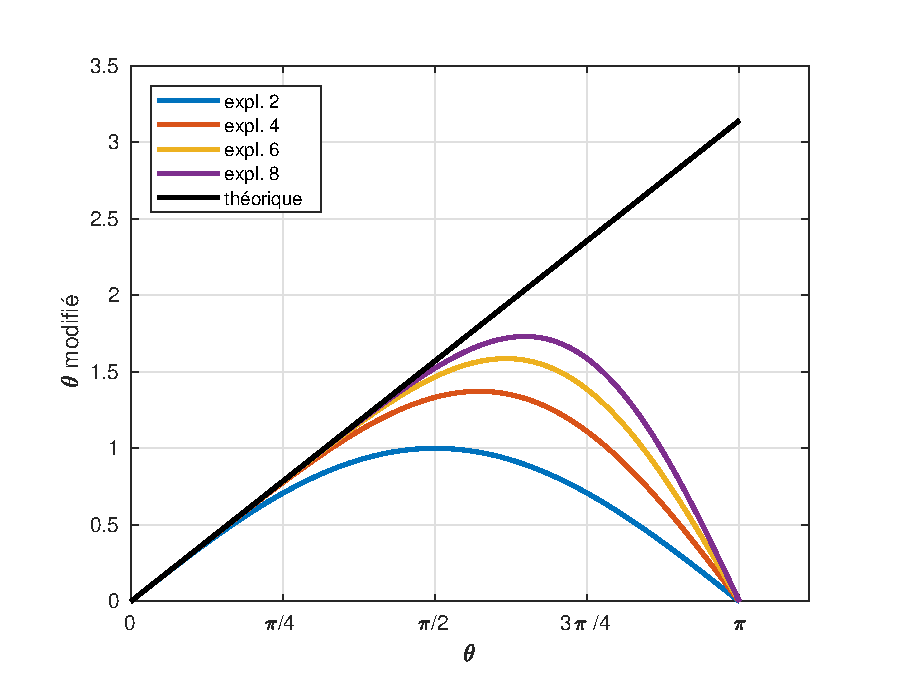
\includegraphics[scale=.6]{freq_classic.eps}
\end{center}
\caption{Représentation de $\theta_m$ en fonction de $\theta$ pour les schémas d'approximation explicites $\delta_{x,P}$ d'ordres 2, 4, 6 et 8.}
\label{fig:freq_classic}
\end{figure}

La figure \ref{fig:freq_classic} permet de constater que les basses fréquences ($k$ petit, donc $\theta$ proche de $0$) sont bien représentées alors que les hautes fréquences ($\theta$ proche de $\pi$) sont mal représentées. En effet lorsque $\theta = \pi$, le nombre $k$ vaut $k = N/2$ et la fonction associée ne peut etre représentée par le maillage. 
Plus l'ordre de précision du schéma est élevée, mieux on représente les hautes fréquences.


L'opérateur $\delta_{P,x}$ est associé à une matrice antisymétrique notée $D_P$.

Les matrices agissent sur $U = [\mathfrak{u}_0, \mathfrak{u}_1, ..., \mathfrak{u}_{N-1}]^T$.
On pose $U_x$ le vecteur $U_x = [\delta_{P,x}\mathfrak{u}_0, \delta_{P,x}\mathfrak{u}_1, ..., \delta_{P,x}\mathfrak{u}_{N-1}]^T$, on a alors :

\begin{equation}
U_x = D_P U
\end{equation}
Les matrices $D_P$ ont les mêmes valeurs propres que $\delta_{x,P}$. $0$ est valeur propre de $D_P$, $D_P$ est non inversible. A titre d'exemple, on donne la matrice associée à l'ordre 2 :

\begin{equation}
D_2 = \dfrac{1}{2h} \begin{bmatrix}
0    & 1    &    &    &     & -1 \\
-1   & 0    & 1  &    & (0) &    \\
     & -1   & 0  & 1  &     &    \\
     &      & \ddots  & \ddots  & \ddots    &    \\
     & (0)  &    & -1 & 0   & 1  \\
1    &      &    &    & -1  & 0  \\
\end{bmatrix}
\end{equation}
dont les vecteurs propres sont 

\begin{equation}
\mu^k = \dfrac{i}{h} \sin \left( \dfrac{2 \pi k}{N} \right). 
\end{equation}
En particulier, on remarque que $\mu^N = 0$. En général, la matrice $D_P$ est donnée par :
\begin{equation}
\left( D_P \right)_{i,j} = \dfrac{1}{2h} \left\lbrace
\begin{array}{ll}
\dfrac{a_p}{p} & \text{ si } j - i \equiv p [N] \text{ avec } 1 \leq p \leq P \\
-\dfrac{a_p}{p} & \text{ si } i - j \equiv p [N] \text{ avec } 1 \leq p \leq P \\
0 & \text{ sinon.}
\end{array}
\right.
\label{eq:matrice_Dp}
\end{equation}











\subsection{Opérateurs Hermitiens périodiques 1D}

Dans son article \cite{Lele1991}, S. K. Lele présente une méthode permettant d'approcher la dérivée en un point en ajoutant une partie implicite au schéma de la forme \eqref{eq:explicite_dx}. Dans ce chapitre, nous ne considérons que les schémas à 3 points implicites. Définissons l'opérateur $\sigma_{3,x}$ par :

\begin{equation}
(\sigma_{3,x} \mathfrak{u})_j = \alpha \mathfrak{u}_j + \beta \left( \mathfrak{u}_{j+1} + \mathfrak{u}_{j-1} \right)
\end{equation}

\begin{theoreme}
Si les coefficients réels $\alpha$, $\beta$ ainsi que les coefficients $(a_i)_{1 \leq i \leq P}$ sont solutions de 
\begin{equation}
\left\lbrace
\begin{array}{rcl}
\gsum_{p=0}^P a_p & = & \alpha + 2 \beta \\
\gsum_{p=0}^P a_p \dfrac{p^{2n}}{2n+1} & = & 2 \beta  \text{ pour } n=1,2,...P
\end{array}
\right.
\label{eq:hermitian_system}
\end{equation}
et si $u$ est une fonction de $\mathcal{C}^{2P+3}$, alors pour tout $0 \leq i \leq N-1$, on a 
\begin{multline}
(\delta_{P,x} u^*)_i - (\sigma_{3,x} u'^*)_i = \\
h^{2P+2} \left( \gsum_{p=0}^P a_p  \dfrac{(j)^{2P+2}}{2(2P+3)!} \left( u^{(2P+3)}(\xi_j) + u^{(2P+3)}(\eta_j) \right) - \dfrac{\beta}{(2P+2)!} \left(u^{(2P+3)}(\varrho) + u^{(2P+3)}(\sigma) \right) \right)
\end{multline}
\end{theoreme}

\begin{proof}
Soit $u : x \in \Omega \mapsto u(x) \in \mathbb{R}$ une fonction de classe $\mathcal{C}^{2P+3}( \Omega)$ et $u^*$ la fonction de grille correspondante.

On considère les développements de Taylor :
\begin{equation}
\begin{array}{rcl}
u(x_i + ph) & = & u(x_i) + p h u'(x_j) + \cdots + \dfrac{(ph)^k}{k!}u^{(k)}(x_i) + \cdots +\dfrac{(ph)^{2P+3}}{(2P+3)!} u^{(2P+3)}(\xi_p)\\
u(x_i - ph) & = & u(x_i) - p h u'(x_j) + \cdots + \dfrac{(-ph)^k}{k!}u^{(k)}(x_i) + \cdots +\dfrac{(-ph)^{2P+3}}{(2P+3)!} u^{(2P+3)}(\eta_p)
\end{array}
\end{equation}
avec $\xi_p \in [x_i, x_i+ph]$ et $\eta_p \in [x_i-ph, x_i]$. En combinant ces deux égalités, on a
\begin{equation}
\dfrac{\tau_pu^*_i - \tau_{-p} u^*_i}{2ph} = u'(x_i) + \cdots + \dfrac{(ph)^{k-1}(1 - (-1)^k)}{2 \cdot k!} u^{(k)}(x_i) + \cdots +\dfrac{(ph)^{2P+2}}{2(2P+3)!} \left( u^{(2P+3)}(\xi_p) + u^{(2P+3)}(\eta_p) \right)
\label{eq:preuve_herm1}
\end{equation}

D'autres part, on a 
\begin{equation}
\alpha u'^*_i + \beta \left( \tau_1 u'^*_{i} + \tau_{-1} u'^*_{i} \right) = (\alpha + 2 \beta) u'^*_i \gsum_{k=1}^{2P+1} \beta \dfrac{h^{k}}{k!} \left( 1 + (-1)^k \right) u^{(k+1)}(x_i)+ \beta \dfrac{h^{2P+2}}{(2P+2)!} \left(u^{(2P+3)}(\varrho) + u^{(2P+3)}(\sigma) \right) 
\label{eq:preuve_herm2}
\end{equation}
avec $\varrho \in [x_i, x_i + h]$ et $\sigma \in [x_i, x_i - h]$. 

On remarque directement que \eqref{eq:preuve_herm2} et $\gsum_{p=0}^P a_p  \eqref{eq:preuve_herm1}$ coïncident pour les puissances de $h$ impaires. 

Pour les autres valeurs, l'égalité est vrai si les coefficients $a_p$, $\alpha$ et $\beta$ sont solutions de \eqref{eq:hermitian_system}. L'erreur de troncature prend directement la forme 

\begin{multline}
(\delta_{P,x} u^*)_i - (\sigma_{3,x} u'^*)_i = \\
h^{2P+2} \left( \gsum_{p=0}^P a_p  \dfrac{(j)^{2P+2}}{2(2P+3)!} \left( u^{(2P+3)}(\xi_j) + u^{(2P+3)}(\eta_j) \right) - \dfrac{\beta}{(2P+2)!} \left(u^{(2P+3)}(\varrho) + u^{(2P+3)}(\sigma) \right) \right)
\end{multline}
\end{proof}

On peut noter que comme $u \in \mathcal{C}^{2P+3}(\Omega)$, alors 
\begin{equation}
\|u^{(2P+3)} \|_{\infty} < \infty
\end{equation}
donc 
\begin{equation}
\| (\delta_{P,x}u^*)_i - (\sigma_{3,x} u'^*)_i \|_{\infty} \leq C \|u^{(2P+3)} \|_{\infty} h^{2P+2} = \mathcal{O}(h^{2P+2})
\label{eq:eq_cons}
\end{equation}

Sous forme matricielle, l'opérateur $\sigma_{3,x}$ s'écrit :
\begin{equation}
S = \begin{bmatrix}
\alpha    & \beta    &    &    &     & \beta \\
\beta   & \alpha    & \beta  &    & (0) &    \\
     & \beta   & \alpha  & \beta  &     &    \\
     &      & \ddots  & \ddots  & \ddots    &    \\
     & (0)  &    & \beta & \alpha   & \beta  \\
\beta    &      &    &    & \beta  & \alpha  \\
\end{bmatrix}
\label{eq:matrice_T}
\end{equation}

\begin{proposition}
La matrice $S$ et l'opérateur $\sigma_{3,x}$ ont pour valeurs propres 
\begin{equation}
\mu^k = \alpha + 2 \beta \cos \left( \dfrac{2 \pi k}{N} \right)
\end{equation}
Chaque valeur propre est associée à un vecteur propre $U^k$ avec $0 \leq k \leq N-1$ et 
\begin{equation}
U^k_j = \exp \left[ ij \dfrac{2 \pi k}{N} \right]
\end{equation}
\label{prop:eigen_implicit_herm}
\end{proposition}

\begin{proof}
Conséquence de la proposition \ref{prop:eigen_tau}. 
\end{proof}

\begin{corollaire}
L'opérateur $\sigma_{3,x}$ est inversible si 
\begin{equation}
\begin{vmatrix}
\dfrac{\alpha}{2 \beta}
\end{vmatrix} > 1.
\end{equation}
De plus, sous cette hypothèse, la matrice $S$ est symétrique définie.
\end{corollaire}

\begin{proof}
Il suffit de vérifier que 
\begin{equation}
| \alpha + 2 \beta \cos \left( \theta \right) | > 1
\end{equation}
pour déduire que les valeurs propres de $\sigma_{3,x}$ sont strictement positive, la symétrie de $S$ est triviale.
\end{proof}

Les opérateurs $\sigma_{3,x}$ considérés dans la suite vérifieront l'hypothèse 
\begin{equation}
\begin{vmatrix}
\dfrac{\alpha}{2 \beta}
\end{vmatrix} > 1.
\end{equation}

\begin{definition}
On définit $\delta_{P,x}^H$ l'\textit{opérateur hermitien} donné par 
\begin{equation}
\delta_{P,x}^H = \sigma_{3,x}^{-1} \circ \delta_{P,x}.
\end{equation}
\end{definition}

Matriciellement, l'opérateur $\delta_{P,x}^H$ est associé à la matrice $S^{-1} D_P$ où $D_P$ est donnée par \eqref{eq:matrice_Dp} et $T$ donné par \eqref{eq:matrice_T}. Dans la pratique, on ne calcule pas directement cette matrice, si
\begin{equation}
U = \begin{bmatrix}
\mathfrak{u}_1 \\
\mathfrak{u}_2 \\
\vdots \\
\mathfrak{u}_N 
\end{bmatrix} \text{ et } 
U_x = \begin{bmatrix}
\delta_{P,x}\mathfrak{u}_1 \\
\delta_{P,x}\mathfrak{u}_2 \\
\vdots \\
\delta_{P,x}\mathfrak{u}_N 
\end{bmatrix}
\end{equation}
alors on procède en deux étapes :
\begin{enumerate}
\item Calculer le produit matrice vecteur 
\begin{equation}
W = D_P U,
\end{equation}
\item Résoudre le système\footnote{La résolution de ce système peut se faire grâce à la formule de Shermann-Morisson-Woodbury couplée à l'algorithme de Thomas.} 
\begin{equation}
S U_x = W.
\end{equation}
\end{enumerate}

\begin{theoreme}
Si $u : x \in \Omega \mapsto u(x) \in \mathbb{R}$ est une fonction de classe $\mathcal{C}^{(2P+3)}$.
Si les coefficients $\alpha$, $\beta$ et $(a_i)_{1 \leq i \leq P}$ sont solutions de \eqref{eq:hermitian_system} et si 
\begin{equation}
\begin{vmatrix}
\dfrac{\alpha}{2 \beta}
\end{vmatrix} > 1.
\end{equation}
Alors 
\begin{equation}
\| u'^* - \delta_{P,x}^H u^* \|_{\infty} \leq C h^{2P+2} \| u^{(2P+3)} \|_{\infty}
\end{equation}
où $C$ est une constante indépendante de $u$.
\end{theoreme}

\begin{proof}
Par calcul immédiat, on a :
\begin{equation}
\begin{array}{rcl}
\|  u'^* - \delta_{P,x}^H u^* \|_{\infty} &=& \| \sigma_{3,x}^{-1} \circ \left( \sigma_{3,x} u'^*  - \delta_{P,x}u^*\right) \|_{\infty}\\
                                      &\leq& \| \sigma_{3,x}^{-1} \|_{\infty} \| \sigma_{3,x} u'^*  - \delta_{P,x}u^*\|_{\infty}\\
                                      &\leq& C h^{2P+2}  \| u^{(2P+3)} \|_{\infty}
\end{array}
\end{equation}
en utilisant $\sigma_{3,x}$ inversible et l'équation \eqref{eq:eq_cons}.
\end{proof}
Quelques exemples de schémas compacts sont donnés dans le corollaire suivant.
\begin{corollaire}
Soit $u : x \in \Omega \mapsto u(x) \in \mathbb{R}$ alors 
\begin{itemize}
\item Si $u \in \mathcal{C}^{5}(\Omega)$ alors 
\begin{equation}
\begin{array}{rcccl}
\sigma_{x} &=& \sigma_{3,x} &=& \dfrac{4}{6} id + \dfrac{1}{6} \left( \tau_1 + \tau_{-1} \right)\\
\delta_{x} &=& \dfrac{\tau_1 - \tau_{-1}}{2h} &&\\ 
\end{array}
\label{eq:comp4}
\end{equation}
et $\delta^H_x = \sigma_x^{-1} \circ \delta_x$ définit un opérateur d'approximation de la dérivée première à l'ordre 4,

\item Si $u \in \mathcal{C}^{7}(\Omega)$ alors 
\begin{equation}
\begin{array}{rcl}
\sigma_{3,x} &=& id + \dfrac{1}{3}\left( \tau_1 + \tau_{-1} \right) \\
\delta_{3,x} &=& \dfrac{14}{9} \dfrac{\tau_1 - \tau_{-1}}{2h} + \dfrac{1}{18} \dfrac{\tau_2 - \tau_{-2}}{4h}\\ 
\end{array}
\label{eq:comp6}
\end{equation}
et $\delta^H_{2,x} = \sigma_{3,x}^{-1} \circ \delta_{2,x}$ définit un opérateur d'approximation de la dérivée première à l'ordre 6,


\item Si $u \in \mathcal{C}^{9}(\Omega)$ alors 
\begin{equation}
\begin{array}{rcl}
\sigma_{3,x} &=& id + \dfrac{3}{8}\left( \tau_1 + \tau_{-1} \right) \\
\delta_{3,x} &=& \dfrac{25}{16} \dfrac{\tau_1 - \tau_{-1}}{2h} + \dfrac{1}{5} \dfrac{\tau_2 - \tau_{-2}}{4h} + \dfrac{1}{80} \dfrac{\tau_3 - \tau_{-3}}{6h} \\ 
\end{array}
\label{eq:comp8}
\end{equation}
et $\delta^H_{3,x} = \sigma_{3,x}^{-1} \circ \delta_{3,x}$ définit un opérateur d'approximation de la dérivée première à l'ordre 8.

\end{itemize}
\end{corollaire}

L'analyse fréquentielle de l'opérateur hermitien $\delta_{P,x}^H$ est basée sur le calcul de ces valeurs propres. Les valeurs propres et les vecteurs propres de $S^{-1} D_P$ sont données par la proposition suivante.

\begin{theoreme}
Les valeurs propres de $S^{-1} D_P$ (et aussi celles de $\delta_{P,x}^H$) sont données par 
\begin{equation}
\varsigma^k = \dfrac{i}{\alpha + 2 \beta \cos \left( \dfrac{2 k \pi}{N} \right)} \left( \gsum_{j=1}^P \dfrac{a_j}{jh} \sin \left( \dfrac{2 k \pi}{N} \right) \right)
\end{equation}
A chaque valeur propre $\varsigma^k$ est associée un vecteur propre $U^k$ donné par 
\begin{equation}
U^k_j = \exp \left[ ij \dfrac{2 \pi k}{N} \right]
\end{equation}
pour $1 \leq j,k \leq N$.
\end{theoreme}

\begin{proof}
On a vu dans la proposition \ref{prop:eigen_implicit_herm} que 
\begin{equation}
S U^k = \left( \alpha + 2\beta \cos \left( \dfrac{2 k \pi}{N} \right) \right) U^k
\end{equation}
donc par passage à l'inverse
\begin{equation}
S^{-1} U^k = \dfrac{1}{\alpha + \beta \cos \left( \dfrac{2 k \pi}{N} \right)} U^k
\end{equation}
De la même manière, on a déjà vu dans le théorème \ref{prop:eigen_explicit} : 
\begin{equation}
D_P U^k = i \left( \gsum_{j=1}^P \dfrac{a_j}{jh} \cos \left( \dfrac{2 k \pi}{N} \right) \right) U^k.
\end{equation}
Par composition
\begin{equation}
S^{-1} D_P U^k = \varsigma^k U^k.
\end{equation}
\end{proof}

Nous supposons que les coefficients $\alpha$, $\beta$ et $(a_j)_{0 \leq j \leq N-1}$ vérifient \eqref{eq:hermitian_system}.
Comme pour les schémas explicites présentés dans la partie précédente, on souhaite comparer la quantité $\theta$ avec
\begin{equation}
\theta_m(\theta) = \dfrac{1}{\alpha + 2 \beta \cos \theta} \left( \gsum_{j=1}^P \dfrac{a_j}{j} \cos j \theta \right)
\end{equation}
Dans l'idéal, on souhaite avoir 
\begin{equation}
\theta \approx \theta_m(\theta)
\end{equation}
au voisinage de $\theta = 0$. Il es déjà facile de voir que 
\begin{equation}
\theta_m(0) = \theta_m(\pi) = 0
\end{equation}
ainsi que de voir que 
\begin{equation}
\theta_m(\theta) = \theta + \mathcal{O}(\theta^{20+2})
\end{equation}
Si l'on trace les nombres $\theta_m$ issus des schémas compacts d'ordre 4, 6 et 8 (équation \eqref{eq:comp4}, \eqref{eq:comp6} et \eqref{eq:comp8}) avec ceux explicites d'ordre 2, 4, 6 et 8, on obtient la figure \ref{fig:freq_comp}.

\begin{figure}[htbp]
\begin{center}
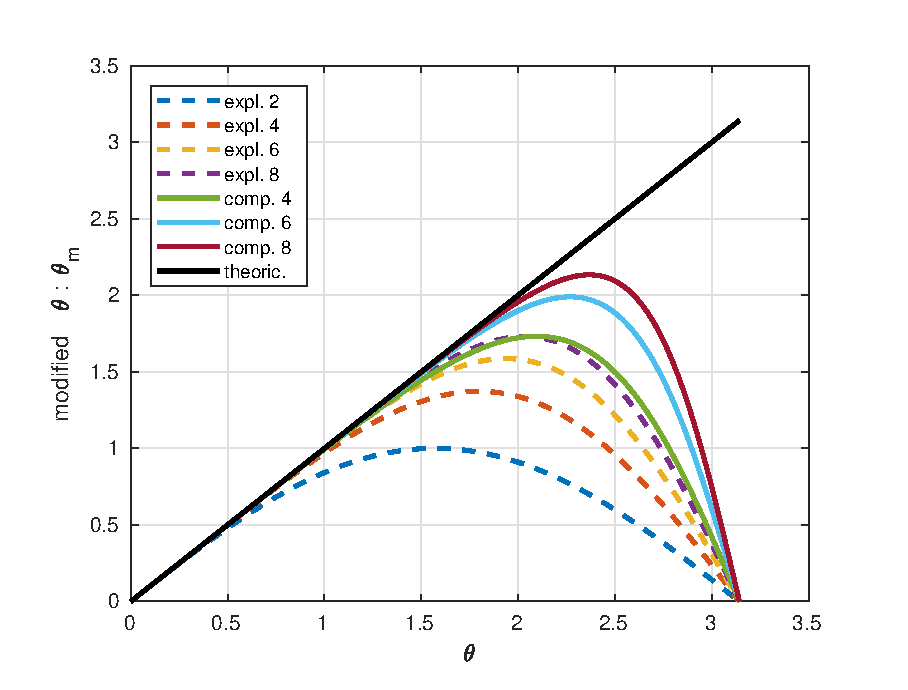
\includegraphics[scale=.6]{freq_total.eps}
\end{center}
\caption{Représentation de $\theta_m$ en fonction de $\theta$ pour les schémas d'approximation explicites $\delta_{x,P}$ d'ordres 2, 4, 6 et 8 (en pointillés) et les schémas compacts $\delta_{x,P}^H$ d'ordres 4, 6 et 8 (en trait plein).}
\label{fig:freq_comp}
\end{figure}
Plusieurs choses sont à remarquer :
\begin{itemize}
\item De manière générale, les schémas compacts représentent mieux les hautes fréquences (lorsque $\theta$ grandit),
\item Plus un schéma est d'ordre élevé, mieux il représente les fréquences.
\end{itemize}














\subsection{Schéma décentré au bord}




























\section{Opérateur de filtrage en dimension 1}

Lors de la discrétisation via un schéma aux différences finies et suite à la discrétisation en temps, des oscillations parasites peuvent apparaître. Il s'agit de phénomènes haute fréquences qu'il est utile de supprimer à l'aide d'un filtre passe-bas. 

Si $\mathfrak{u}$ est une fonction de grille périodique, on note le filtre passe-bas $\mathcal{F}\mathfrak{u}$. Dans la pratique, nous cherchons $\mathcal{F}$ sous la forme 

\begin{equation}
\mathcal{F} = \gsum_{k=0}^F a_k \dfrac{\tau_k + \tau_{-k}}{2}
\end{equation}
Il s'agit d'un filtre centré en espace.
Il est important de déterminer les conditions que doivent vérifier les coefficients $(a_k)_{0\leq k \leq F}$ pour définir un filtre approprié. Ainsi, si $u : x \in \Omega \mapsto u(x) \in \mathbb{R}$ est une fonction périodique, on note $u^*$ la fonction de grille associée.
Un tel filtre doit 
\begin{itemize}
\item être consistant avec la donnée initiale (hypothèse de consistance),
\item perturber le moins possible la donnée initiale (hypothèse de précision),
\item supprimer ou atténuer les hautes fréquences (hypothèse de filtrage).
\end{itemize}



















\section{Opérateurs d'interpolation}


\section{Discrétisation temporelle}


FAIRE ICI L'ETUDE CLASSIQUE DES METHODES DE RUNGE-KUTTA MAIS EXCLUSIVEMENT POUR RK4.
CE N'EST PAS UN TRAITÉ SUR LES RK ET JE N'UTILISE QUE RK4.
JE PENSE QUE C'EST MIEUX COMME CA.
